%%%%%%%%%%%%%%%%%%%%%%%%%%%%%%%%%%%%%%%%%
% Programming/Coding Assignment
% LaTeX Template
%
% This template has been downloaded from:
% http://www.latextemplates.com
%
% Original author:
% Ted Pavlic (http://www.tedpavlic.com)
%
% Note:
% The \lipsum[#] commands throughout this template generate dummy text
% to fill the template out. These commands should all be removed when 
% writing assignment content.
%
% This template uses a Perl script as an example snippet of code, most other
% languages are also usable. Configure them in the "CODE INCLUSION 
% CONFIGURATION" section.
%
%%%%%%%%%%%%%%%%%%%%%%%%%%%%%%%%%%%%%%%%%

%----------------------------------------------------------------------------------------
%	PACKAGES AND OTHER DOCUMENT CONFIGURATIONS
%----------------------------------------------------------------------------------------

\documentclass{article}

\usepackage{fancyhdr} % Required for custom headers
\usepackage{lastpage} % Required to determine the last page for the footer
\usepackage{extramarks} % Required for headers and footers
\usepackage[usenames,dvipsnames]{color} % Required for custom colors
\usepackage{graphicx} % Required to insert images
\usepackage{listings} % Required for insertion of code
\usepackage{courier} % Required for the courier font
\usepackage{lipsum} % Used for inserting dummy 'Lorem ipsum' text into the template

\usepackage{float}
\usepackage{amsfonts}
\usepackage{amsmath}
\usepackage{bm}

% Margins
\topmargin=-0.45in
\evensidemargin=0in
\oddsidemargin=0in
\textwidth=6.5in
\textheight=9.0in
\headsep=0.25in

\linespread{1.1} % Line spacing

% Set up the header and footer
\pagestyle{fancy}
\lhead{K. Holmbeck and D. Tonne} % Top left header
\chead{\hmwkClass\ : \hmwkTitle} % Top center head
\rhead{\firstxmark} % Top right header
\lfoot{\lastxmark} % Bottom left footer
\cfoot{} % Bottom center footer
\rfoot{Page\ \thepage\ of\ \pageref{LastPage}} % Bottom right footer
\renewcommand\headrulewidth{0.4pt} % Size of the header rule
\renewcommand\footrulewidth{0.4pt} % Size of the footer rule

\setlength\parindent{0pt} % Removes all indentation from paragraphs

%----------------------------------------------------------------------------------------
%	CODE INCLUSION CONFIGURATION
%----------------------------------------------------------------------------------------

\usepackage{color} %red, green, blue, yellow, cyan, magenta, black, white
\definecolor{mygreen}{RGB}{28,172,0} % color values Red, Green, Blue
\definecolor{mylilas}{RGB}{170,55,241}

\lstset{language=Matlab,%
    basicstyle=\ttfamily\footnotesize,breaklines=true
    %basicstyle=\footnotesize\color{red},
    breaklines=true,%
    xleftmargin=0.5in,
    %xrightmargin=0.25in,
    morekeywords={matlab2tikz},
    keywordstyle=\color{blue},%
    morekeywords=[2]{1}, keywordstyle=[2]{\color{black}},
    identifierstyle=\color{black},%
    stringstyle=\color{mylilas},
    commentstyle=\color{mygreen},%
    showstringspaces=false,%without this there will be a symbol in the places where there is a space
    numbers=left,%
    numberstyle={\tiny \color{black}},% size of the numbers
    numbersep=9pt, % this defines how far the numbers are from the text
    emph=[1]{for,end,break},emphstyle=[1]\color{blue}, %some words to emphasise
    %emph=[2]{word1,word2}, emphstyle=[2]{style},    
}


%----------------------------------------------------------------------------------------
%	DOCUMENT STRUCTURE COMMANDS
%	Skip this unless you know what you're doing
%----------------------------------------------------------------------------------------

% Header and footer for when a page split occurs within a problem environment
\newcommand{\enterProblemHeader}[1]{
%\nobreak\extramarks{#1}{#1 continued on next page\ldots}\nobreak
%\nobreak\extramarks{#1 (continued)}{#1 continued on next page\ldots}\nobreak
}

% Header and footer for when a page split occurs between problem environments
\newcommand{\exitProblemHeader}[1]{
\nobreak\extramarks{#1 (continued)}{#1 continued on next page\ldots}\nobreak
\nobreak\extramarks{#1}{}\nobreak
}

\setcounter{secnumdepth}{0} % Removes default section numbers
\newcounter{homeworkProblemCounter} % Creates a counter to keep track of the number of problems

\newcommand{\homeworkProblemName}{}
\newenvironment{homeworkProblem}[1][Problem \arabic{homeworkProblemCounter}]{ % Makes a new environment called homeworkProblem which takes 1 argument (custom name) but the default is "Problem #"
\stepcounter{homeworkProblemCounter} % Increase counter for number of problems
\renewcommand{\homeworkProblemName}{#1} % Assign \homeworkProblemName the name of the problem
\subsection{\homeworkProblemName} % Make a section in the document with the custom problem count
\enterProblemHeader{\homeworkProblemName} % Header and footer within the environment
}{
\exitProblemHeader{\homeworkProblemName} % Header and footer after the environment
}

\newcommand{\problemAnswer}[1]{ % Defines the problem answer command with the content as the only argument
\noindent\framebox[\columnwidth][c]{\begin{minipage}{0.98\columnwidth}#1\end{minipage}} % Makes the box around the problem answer and puts the content inside
}

\newcommand{\homeworkSectionName}{}
\newenvironment{homeworkSection}[1]{ % New environment for sections within homework problems, takes 1 argument - the name of the section
\renewcommand{\homeworkSectionName}{#1} % Assign \homeworkSectionName to the name of the section from the environment argument
\subsection{\homeworkSectionName} % Make a subsection with the custom name of the subsection
\enterProblemHeader{\homeworkProblemName\ [\homeworkSectionName]} % Header and footer within the environment
}{
\enterProblemHeader{\homeworkProblemName} % Header and footer after the environment
}


%----------------------------------------------------------------------------------------
%   NAME AND CLASS SECTION
%----------------------------------------------------------------------------------------

\newcommand{\hmwkTitle}{Homework\ 3} % Assignment title
\newcommand{\hmwkDueDate}{Thursday,\ March\ 22,\ 2018} % Due date
\newcommand{\hmwkClass}{Math\ 521} % Course/clas
\newcommand{\hmwkAuthorName}{Kristin Holmbeck} % Your name

%----------------------------------------------------------------------------------------
%   TITLE PAGE
%----------------------------------------------------------------------------------------

\title{
\textmd{\textbf{\hmwkClass \ \hmwkTitle}}\\
\normalsize\vspace{0.1in}\small{Due\ on\ \hmwkDueDate}\\
\vspace{0.1in}
\vspace{0.2in}
}

\author{\textbf{\hmwkAuthorName}}
\date{} % Insert date here if you want it to appear below your name

%----------------------------------------------------------------------------------------

\begin{document}

\maketitle

%----------------------------------------------------------------------------------------
%   TABLE OF CONTENTS
%----------------------------------------------------------------------------------------

%\setcounter{tocdepth}{1} % Uncomment this line if you don't want subsections listed in the ToC
\vspace{0.75in}
\tableofcontents
\listoffigures
\newpage

%----------------------------------------------------------------------------------------
%   PROBLEM 1
%----------------------------------------------------------------------------------------

% To have just one problem per page, simply put a \clearpage after each problem

\begin{section}{Theory}

\begin{homeworkSection}{1. Gradient of Inner Product}

Show that $\nabla_{\bm{v}} (\bm{v}, \bm{v}) = 2\bm{v}$ and that for a symmetric matrix $C$, $\nabla_{\bm{v}} (\bm{v}, C\bm{v}) = 2C\bm{v}$. 

\problemAnswer{
Assume $\bm{v} \in \mathbb{R}^n$.
	\begin{align*}
		\nabla_{\bm{v}} (\bm{v}, \bm{v}) &= \nabla_{\bm{v}} \bm{v}^T\bm{v} \\
			&= \nabla_{\bm{v}} \left ( v_1^2 + v_2^2 + \cdots + v_n^2 \right ) \\
			&= \left( \frac{\partial \left ( v_1^2 + v_2^2 + \cdots + v_n^2 \right ) }{\partial v_1}, \ldots, \frac{\partial \left ( v_1^2 + v_2^2 + \cdots + v_n^2 \right ) }{\partial v_n}, \right ) \\ 
			&= \left( 2v_1,  2v_2, \ldots, 2v_n \right ) \\
			&= 2 \bm{v}
	\end{align*}
Next, show $\nabla_{\bm{v}} (\bm{v}, C\bm{v}) = 2C\bm{v}$ :
	\begin{align*}
		\text{Let } \bm{v} &= \begin{bmatrix} v_1 \\ v_2 \\ \vdots \\ v_n \end{bmatrix} \\
		\text{and } C &= \begin{bmatrix} c_{11} && c_{12} && \cdots && c_{1n} \\
			c_{21} && c_{22} && \cdots && c_{2n} \\ 
			\vdots && 		&& 			&& \vdots \\
			c_{n1} &&    \cdots && && c_{nn} \end{bmatrix}
			= \begin{bmatrix} c_{11} && c_{21} && \cdots && c_{n1} \\
			c_{12} && c_{22} && \cdots && c_{n2} \\ 
			\vdots && 		&& 			&& \vdots \\
			c_{1n} &&    \cdots && && c_{nn} \end{bmatrix} \\
		&= \begin{bmatrix} \vec{c}_1 \cdots \vec{c}_n \end{bmatrix} \\
		\text{then } \bm{v}^T C\bm{v} &= \begin{bmatrix} v_1 &&  \cdots && v_n \end{bmatrix}
				\begin{bmatrix} \vec{c}_1 \cdot \bm{v} \\ \vdots \\ \vec{c}_n \cdot \bm{v} \end{bmatrix}
			= v_1 \vec{c}_1 \cdot \bm{v} + \cdots + v_ n \vec{c}_n \cdot \bm{v} \\
		&= v_1 (c_{11} v_1 + c_{12} v_2 + \cdots + c_{1n}v_n)  + \cdots + v_n (c_{n1} v_1 + c_{n2} v_2 + \cdots + c_{nn}v_n) \\ 
		\text{So } \nabla_{\bm{v}} (\bm{v}, C\bm{v}) &= \nabla_{\bm{v}} \bm{v}^T C\bm{v} \\
		\nabla_{\bm{v}} \bm{v}^T C\bm{v} &= 
			\begin{bmatrix} \partial v_1 (\bm{v}^T C\bm{v}) \\ \vdots \\ \partial v_n (\bm{v}^T C\bm{v}) \end{bmatrix} \\
		&= \begin{bmatrix} \vec{c}_1 \cdot \bm{v} + \end{bmatrix} \\
		\partial v_k (\bm{v}^T C\bm{v}) &= v1 c_{1k} + v2 c_{2k} + \cdots + \partial v_k \left [ v_k (c_{k1}v1 + \cdots + c_{kk}v_k + \cdots + c_{kn}v_n) \right ] + \cdots + v_n c_{nk}
		\\
		\partial v_k (\bm{v}^T C\bm{v}) &= v1 c_{1k} + v2 c_{2k} + \cdots + \left [ (c_{k1}v1 + \cdots + c_{kk}v_k + \cdots + c_{kn}v_n ) + v_k c_{kk} \right ] + \cdots + v_n c_{nk} \\
		&= 2 \vec{c}_k \bm{v} \\
		\implies \nabla_{\bm{v}} (\bm{v}, C\bm{v}) &= 2 C \bm{v} \\
	\end{align*}
}

\end{homeworkSection}

\begin{homeworkSection}{2. Commutativity of Symmetric Matrix in the Inner Product}
Show that for a symmetric matrix $C$, $( \phi^{(1)}, C\phi^{(2)} ) = ( C\phi^{(1)}, \phi^{(2)} )$.

\problemAnswer{ 
	\begin{align*}
		(x,Cy) &= (Cy)^Tx = y^TC^T x = y^T Cx = (Cx,y) \\
		\implies (x,Cy) &= (Cx,y)
	\end{align*}
}

\end{homeworkSection}


\begin{homeworkSection}{3. Eigenvalues and eigenvectors}
Given the data matrix 
$$ X = \begin{bmatrix} -2 && -1 && 1 \\ 0 && -1 && 0 \\ -1 && 1 && 2 \\ 1 && -1 && 1
\end{bmatrix} $$
compute the eigenvalues and eigenvectors of $XX^T$ and $X^TX$. For $\bm{u}^{(1)}$, confirm the statement
$$
	\bm{u}^{(j)} = \frac{1}{\sigma_j} \Sigma_{k=1}^{P} v_k^{(j)} \bm{x}^{(k)}
$$
\problemAnswer{
	By \textsc{Matlab}, $\rho(XX^T) = \lambda(\lambda - 9)(\lambda - 4)(\lambda-3) = \lambda \rho(X^T X)$, i.e. the eigenvalues of $XX^T$ are $\lbrace 0, 3, 4, 9 \rbrace$ and the eigenvalues of $X^TX$ are $\lbrace 3, 4, 9 \rbrace$. (See the heavy-lifting code at the end of this document). The eigenvectors of $X^TX$ are the column vectors of the matrix:
	\begin{align*}
		\begin{bmatrix}-0.71 && 0.50 && -0.41 && -0.29 \\ 0.00 && 0.50 && -0.00 && 0.87 \\ -0.71 && -0.50 && 0.41 && 0.29 \\ -0.00 && 0.50 && 0.82 && -0.29 \end{bmatrix}
	\end{align*}
	and the eigenvectors of $XX^T$ are the column vectors of
	\begin{align*}
		\begin{bmatrix}-0.71 && 0.00 && -0.71 \\ 0.00 && -1.00 && 0.00 \\ 0.71 && 0.00 && -0.71 \end{bmatrix}
	\end{align*}.
	Note that the matrix eigenvectors of $XX^T$ is the same as the matrix $V$ in the SVD decomposition $X = U \Sigma V^T$, i.e. the eigenvectors of $XX^T$ are the right singular vectors of $X$.
	For $\bm{u}^{(1)}$,
	\begin{align*}
		\frac{1}{\sigma_1} \Sigma_{k=1}^{P} v_k^{(1)} \bm{x}^{(k)}
		&= \frac{1}{3} \left( 
			-0.7071 \begin{bmatrix}-2.00 \\ 0.00 \\ -1.00 \\ 1.00 \end{bmatrix}
			+ 0 \begin{bmatrix}-1.00 \\ -1.00 \\ 1.00 \\ -1.00 \end{bmatrix}
			+ 0.7071 \begin{bmatrix}1.00 \\ 0.00 \\ 2.00 \\ 1.00 \end{bmatrix}
		\right ) \\
		&= \begin{bmatrix}0.71 \\ 0.00 \\ 0.71 \\ -0.00 \end{bmatrix} = \bm{u}^{(1)}
	\end{align*}
	Where the vector $\bm{u}^{(1)}$ is calculated from SVD via \textsc{Matlab}. 
}
\end{homeworkSection}


\begin{homeworkSection}{4. FLOP count}
Assume $A$ is $N \times P$, and that $N > P$. Then the SVD of $A$ is $A=U \Sigma V^T$ where $U$ is $N \times P$, $\Sigma$ is $P\times P$, and $V$ is $P\times P$.

\problemAnswer {
	\begin{align*}
	 A = \Sigma V^T &= 
		 \begin{bmatrix} \sigma_{1} &&  && 0 \\  && \ddots &&  \\ 0 &&  && \sigma_{P} \\ 0 && \cdots && 0 \end{bmatrix}
		 \begin{bmatrix} v_{11} && \cdots && v_{1P} \\ \vdots && \ddots && \vdots \\ v_{P1} && \cdots && v_{PP} \end{bmatrix}^T \\
	&= 	\begin{bmatrix} \sigma_{1} &&  && 0 \\  && \ddots &&  \\ 0 &&  && \sigma_{P} \\ 0 && \		\cdots && 0 \end{bmatrix}
		\begin{bmatrix} v_{11} && \cdots && v_{P1} \\ \vdots && \ddots && \vdots \\ v_{1P} && \cdots && v_{PP} \end{bmatrix} \\
	&= \begin{bmatrix}
		\sigma_1 {\bm{v}^{(1)}}^T  \\
		\sigma_2 {\bm{v}^{(2)}}^T  \\
		\vdots \\
		\sigma_P {\bm{v}^{(P)}}^T  \\
		\end{bmatrix}
	= \begin{bmatrix}
		\text{$P$ scalar multiplies} \\
		\text{$P$ scalar multiplies} \\
		\vdots \\ 
		\text{$P$ scalar multiplies}
		\end{bmatrix}
	= \text{$P^2$ operations}
	\end{align*}
On the other hand,
	\begin{align*}
		A = U^T X &= \begin{bmatrix} u_{11} && \cdots && u_{N1} \\ \vdots && \ddots && \vdots \\ u_{1P} && \cdots && u_{NP} \end{bmatrix}^T 
			 \begin{bmatrix} x_{11} && \cdots && x_{N1} \\ \vdots && \ddots && \vdots \\ x_{1P} && \cdots && x_{NP} \end{bmatrix} \\
		&= \begin{bmatrix} u_{11} && \cdots && u_{P1} \\ \vdots && \ddots && \vdots \\ u_{1N} && \cdots && u_{PN} \end{bmatrix} 
			 \begin{bmatrix} x_{11} && \cdots && x_{N1} \\ \vdots && \ddots && \vdots \\ x_{1P} && \cdots && x_{NP} \end{bmatrix} \\
		&= \begin{bmatrix}
			\text{$P$ multiplies, $P-1$ additions} && \cdots && \text{$P$ multiplies, $P-1$ additions} \\
			\vdots && \ddots && \vdots \\
			\text{$P$ multiplies, $P-1$ additions} && \cdots && \text{$P$ multiplies, $P-1$ additions}
			\end{bmatrix}_{N \times N} \\
		&= \begin{bmatrix}
			\text{$2P-1$ operations} && \cdots && \text{$2P-1$ operations} \\
			\vdots && \ddots && \vdots \\
			\text{$2P-1$ operations} && \cdots && \text{$2P-1$ operations}
			\end{bmatrix}_{N \times N} \\
		&= \text{$(2P-1)N^2$ operations}
	\end{align*}
}
\end{homeworkSection}

\end{section}


\newpage
\begin{section}{Computing}
The computing assignment is to apply the \textit{snapshot} method to a collection of high-resolution files. We will briefly discuss the background being the method, the implementation, and provide results on a test data set.
\\
\\
Suppose we have a set of $P$ $N \times N$ matrices where $P << N$. The KL expansion as discussed in class gives rise to a construction of an optimal basis for a set of vectors $\lbrace{\bm{x}^{(\mu)}} \rbrace_{\mu=1}^P$ characterized by:

\begin{align}
	C \phi^{(i)} &= \lambda_i \phi^{(i)} \label{eqn:KL}
\end{align}
\begin{align*}
	\text{where} \quad C &= \frac{1}{P} \Sigma_{\mu=1}^P (x^{(\mu)} - \langle x \rangle )(x^{(\mu)} - \langle x \rangle )^T \qquad \text{is the ensemble average covariance matrix} \\
	\text{and} \quad \langle x \rangle &= \frac{1}{P} \Sigma_{\mu=1}^P x^{(\mu)} \qquad \text{is the ensemble average}
\end{align*}

Notice that $C$ is $N \times N$. When $N$ becomes large, it is not feasible to solve this problem directly. If $C$ is nonsingular, we can reduce (without approximation) the problem from Equation \ref{eqn:KL} into a $P \times P$ problem. This is known as the $snapshot$ method. We showed in class that we can obtain a best basis for the $C$ matrix from the thin SVD of $X$.

\vspace{10pt}

\problemAnswer{
	\vspace{10pt}
	The test data set in question involves a fixed camera in a room with a person facing the camera and moving in the foreground. The ensemble average of these data is shown in Figure \ref{fig:ensemble_average}.

    \begin{minipage}{1.0\textwidth}
        \begin{figure}[H]
        \centering
        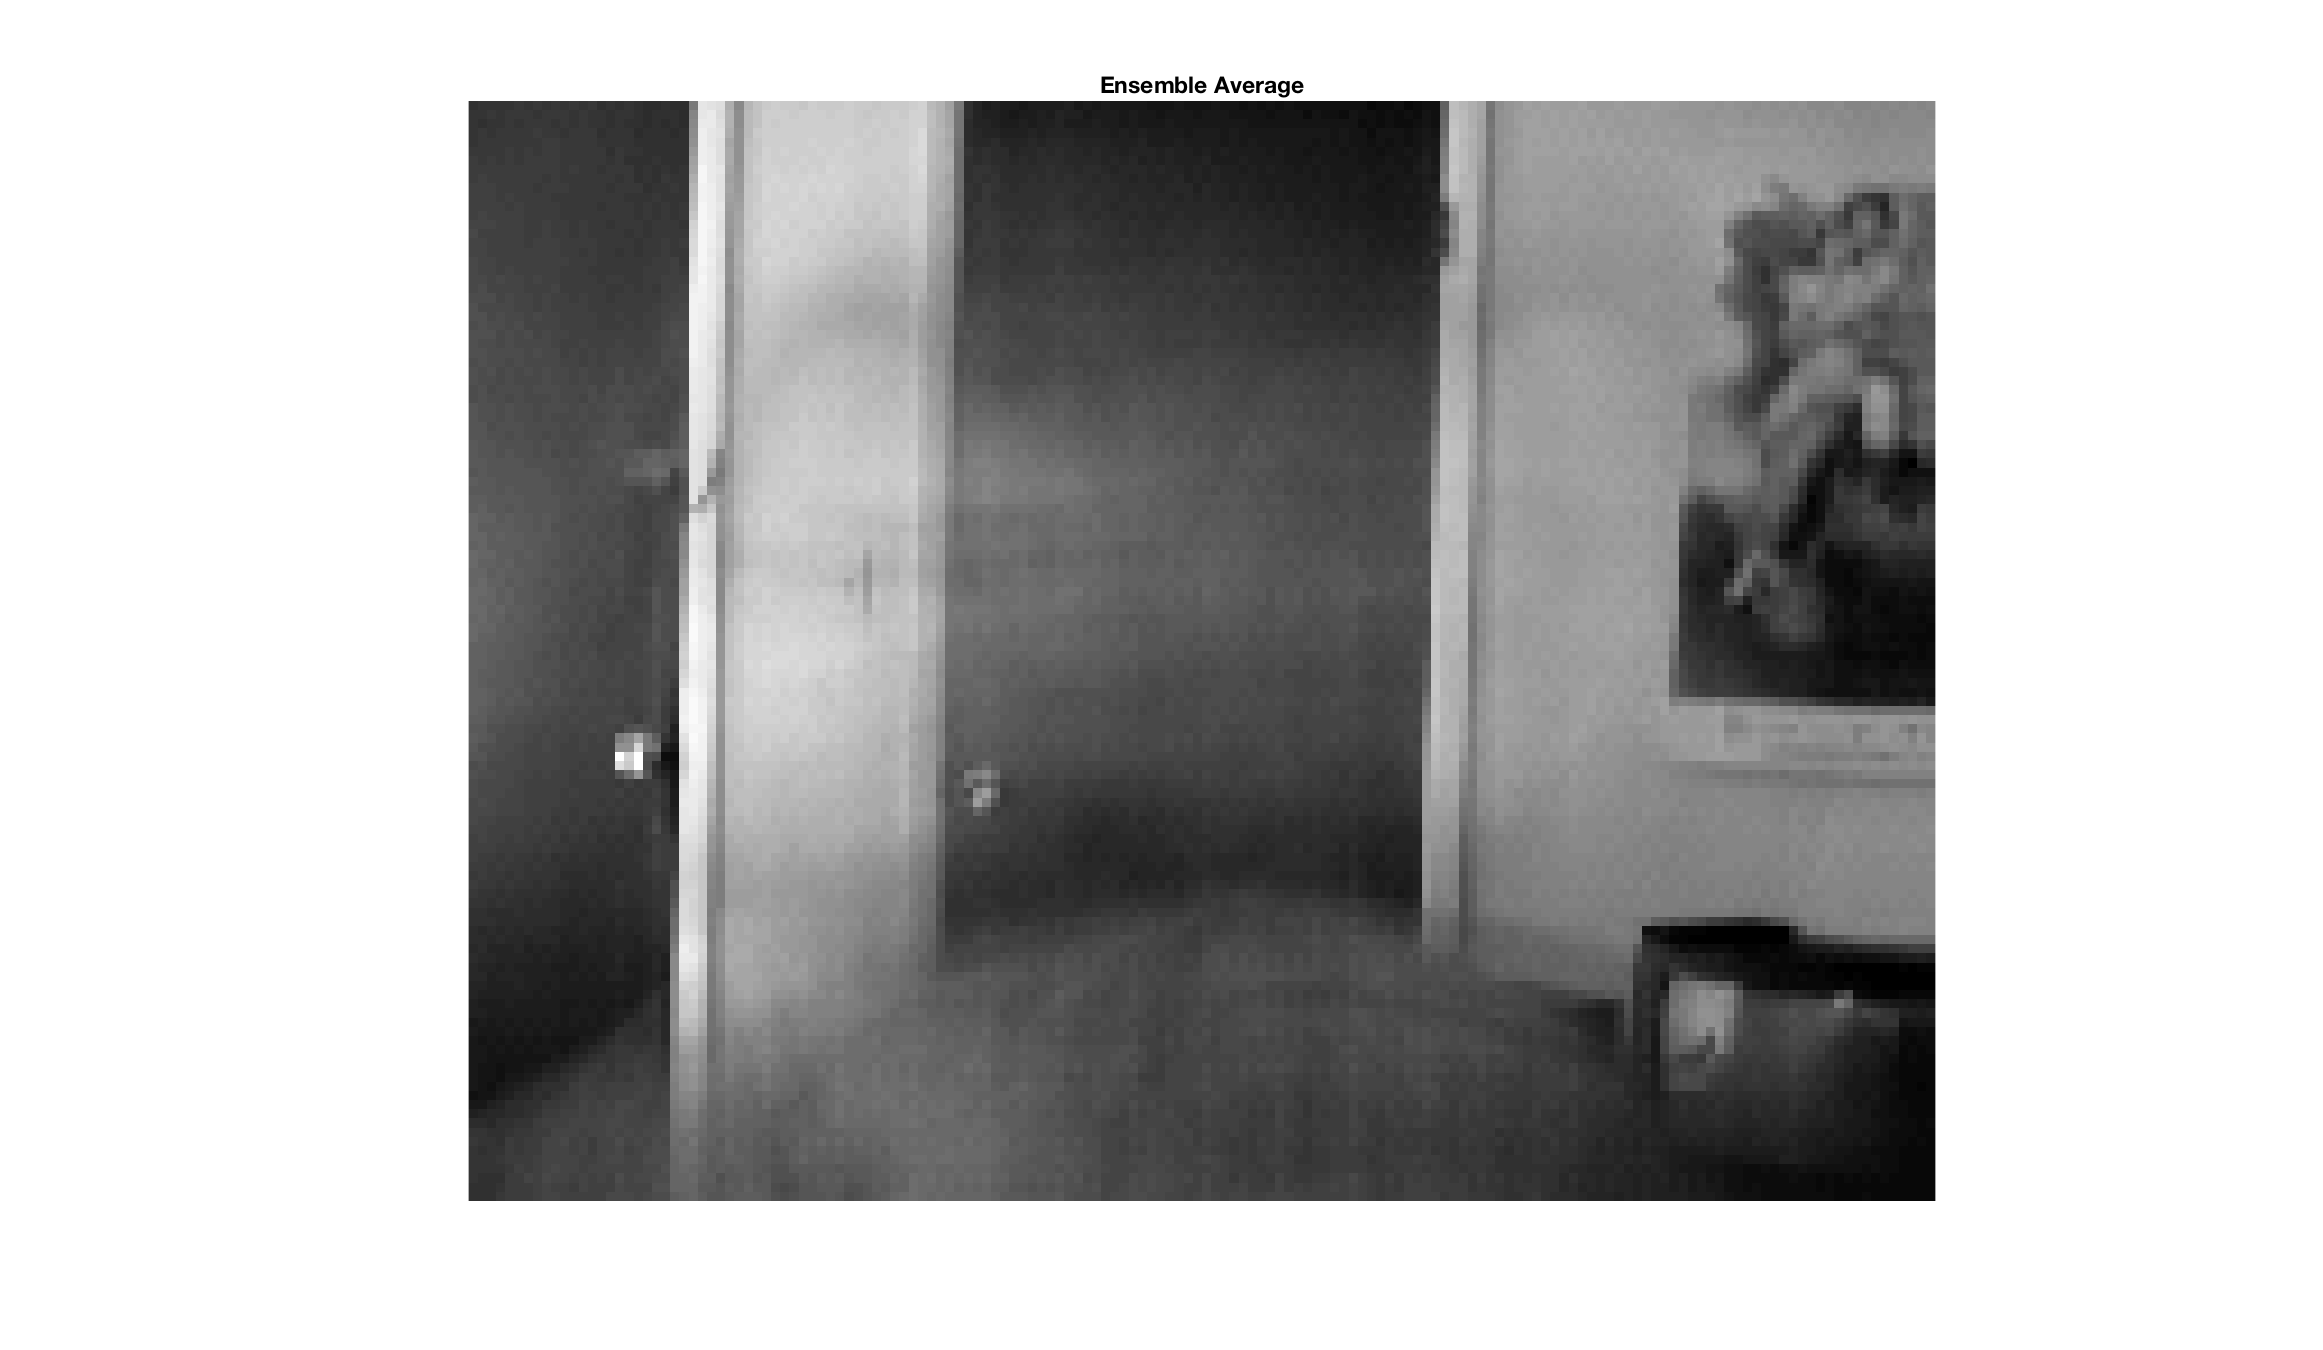
\includegraphics[trim={0cm 2cm 0cm 2cm},clip,width=0.85\columnwidth]{../data/ensemble_average}
        \caption{Ensemble Average of data set}
        \label{fig:ensemble_average}
        \end{figure}
    \end{minipage}
}
\problemAnswer{
	\vspace{10pt}
	Next, we display one of the mean-subtracted images, that is, the data set minus the ensemble average (Figure \ref{fig:mean_subtracted_ex}). \\
    \begin{minipage}{1.0\textwidth}
        \begin{figure}[H]
        \centering
        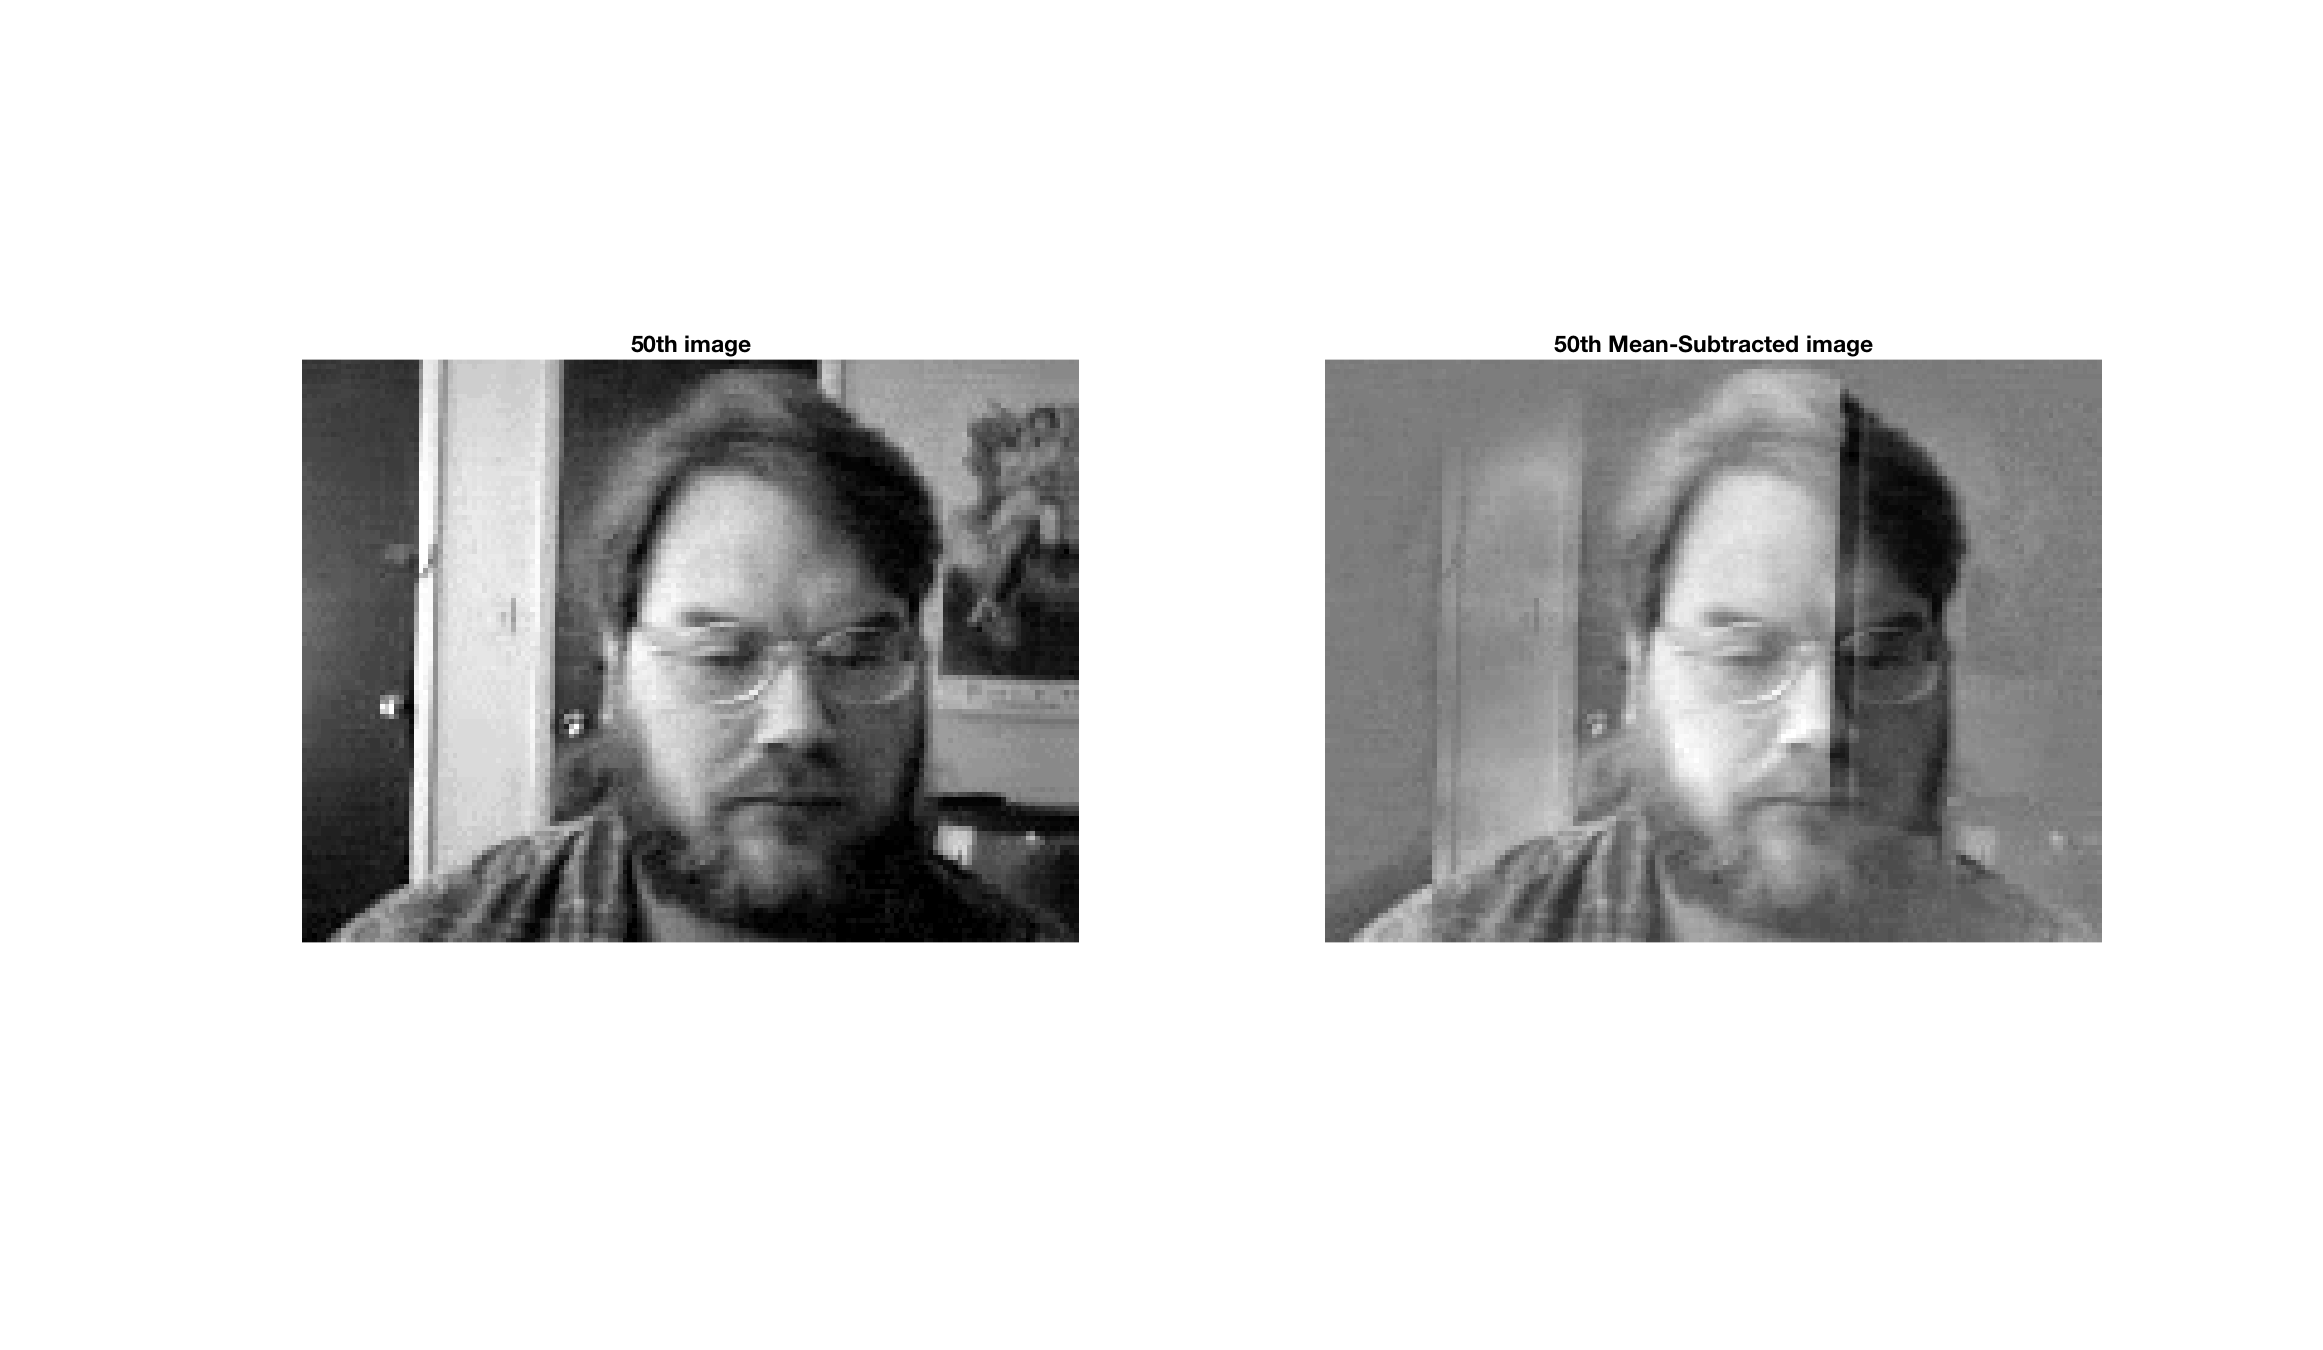
\includegraphics[trim={2cm 3cm 2cm 3cm},clip,width=0.85\columnwidth]{../data/mean_subtracted_ex}
        \setlength{\belowcaptionskip}{15pt}
        \caption{50th mean-subtracted image}
        \label{fig:mean_subtracted_ex}
        \end{figure}
    \end{minipage}
    \\
    Additionally, several eigen-images are shown below:

    \begin{minipage}{1.0\textwidth}
        \begin{figure}[H]
        \centering
        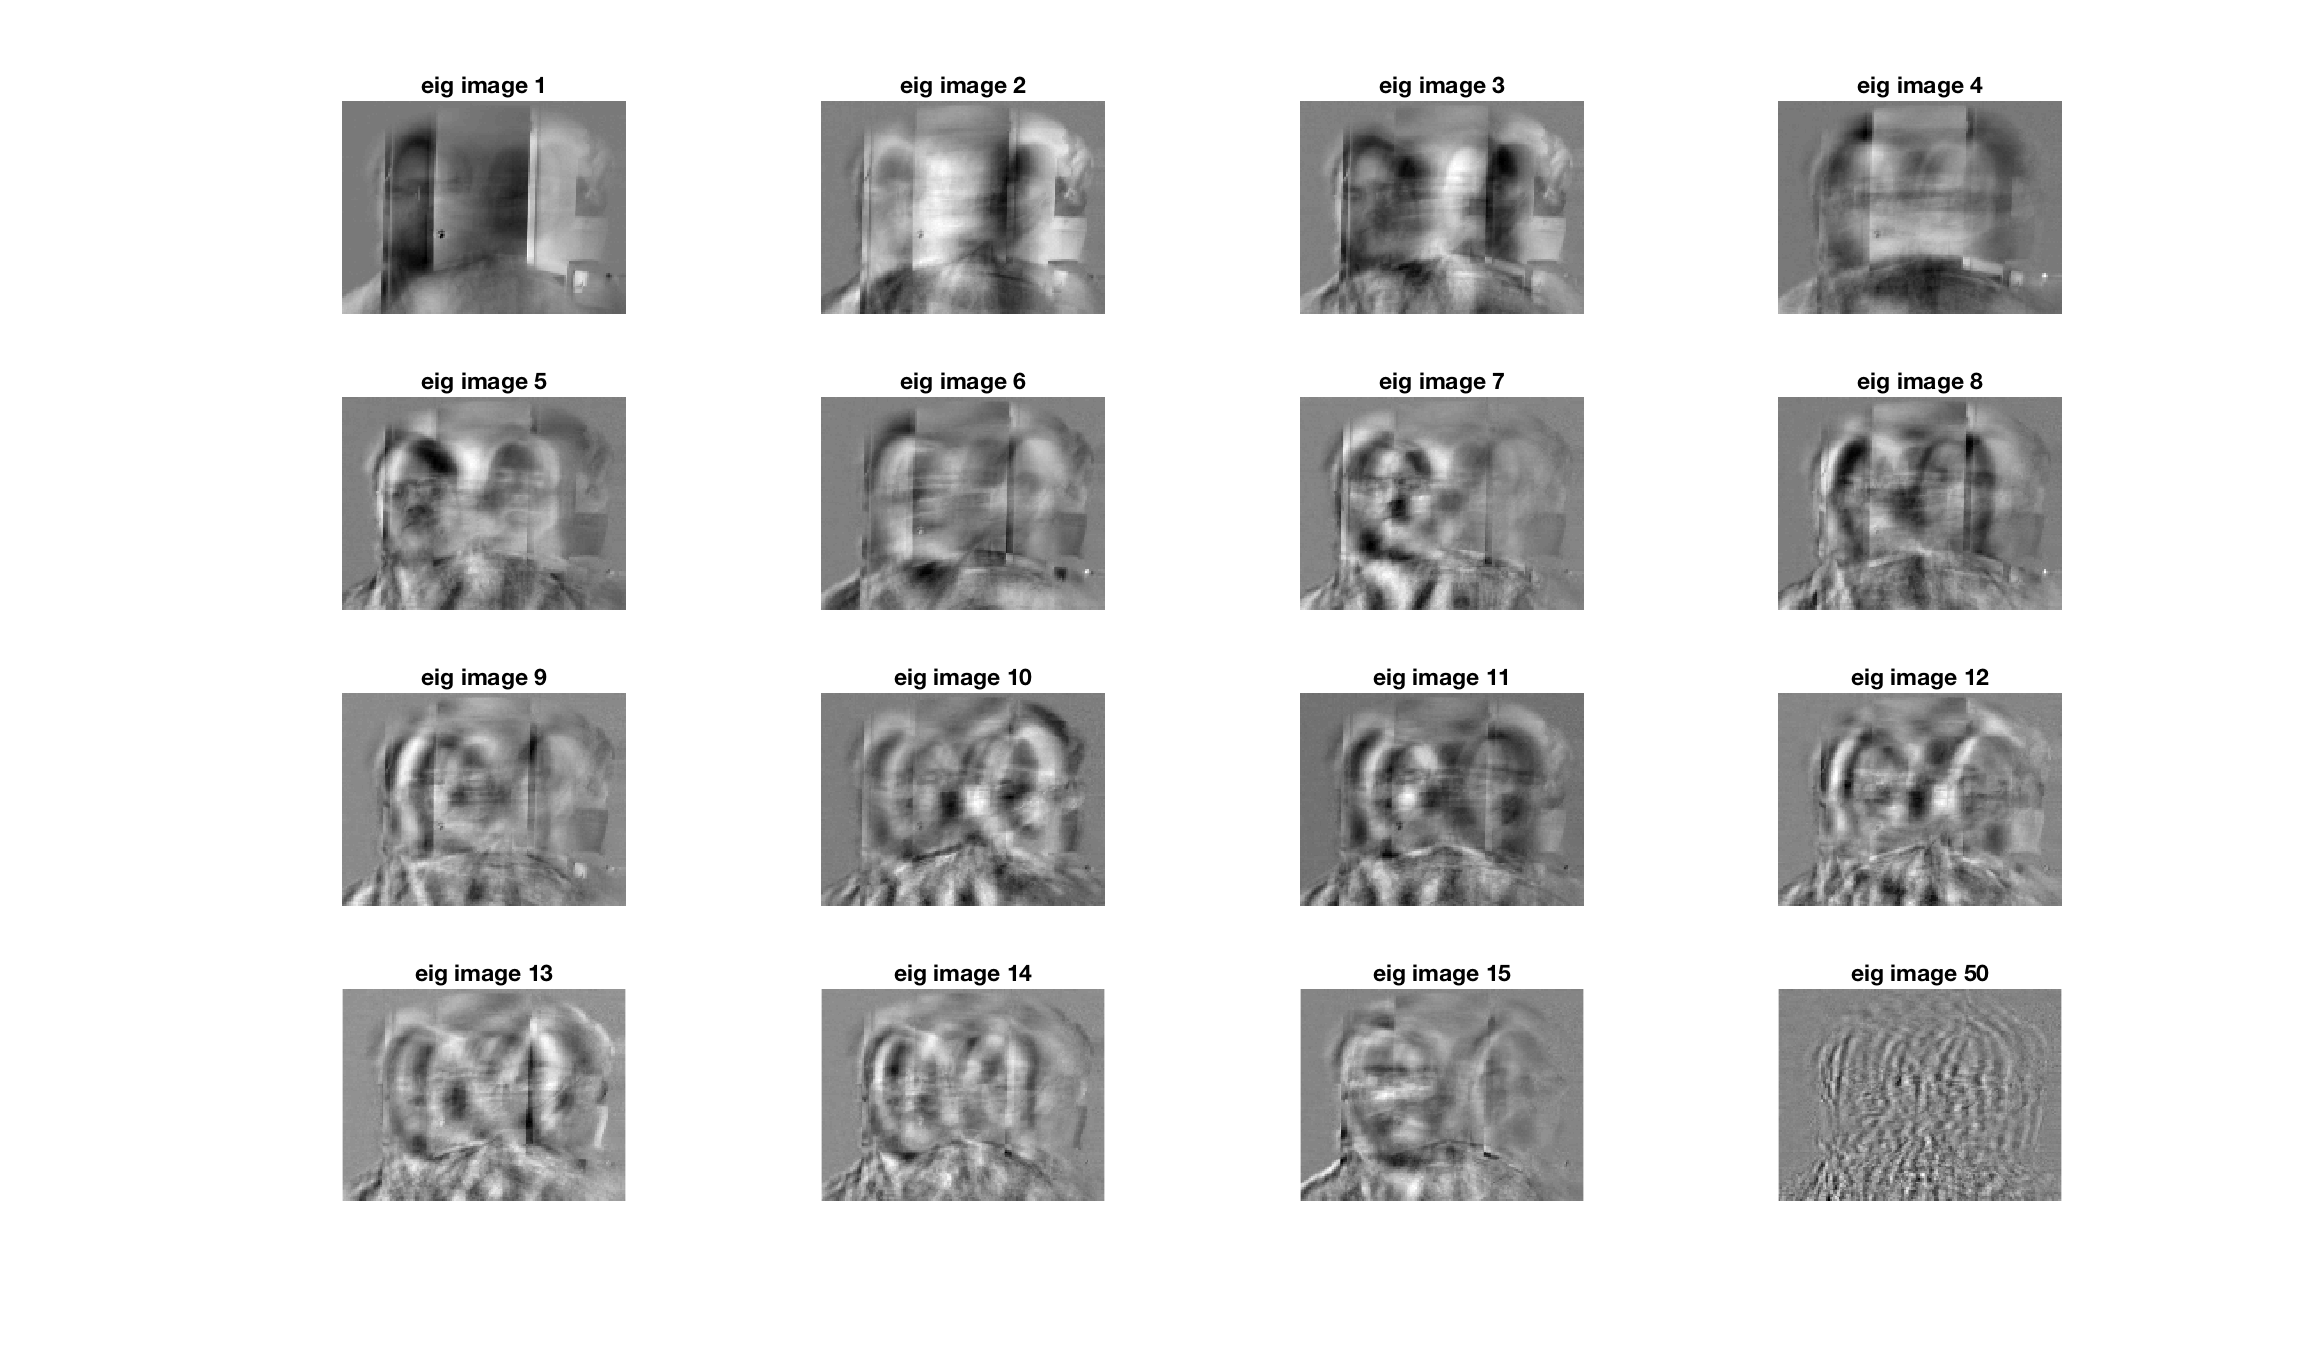
\includegraphics[trim={0cm 0cm 0cm 2cm},clip,width=0.85\columnwidth]{../data/eig_images}
        \setlength{\abovecaptionskip}{-20pt}
        \caption{Some eigen-images}
        \label{fig:eig_images}
        \end{figure}
    \end{minipage}
    \\
    \\
    \\
	The graph in Figure \ref{fig:eigvals} shows the scaled singular values in order. We can use this as a way to determine where the cutoff rank should be. For example, at the ``elbow" of the curve.
	\\
	\\
}

\problemAnswer{
	Below we present a few reconstructions for the 50-th image from Figure \ref{fig:mean_subtracted_ex}.
        \begin{figure}[H]
        \centering
        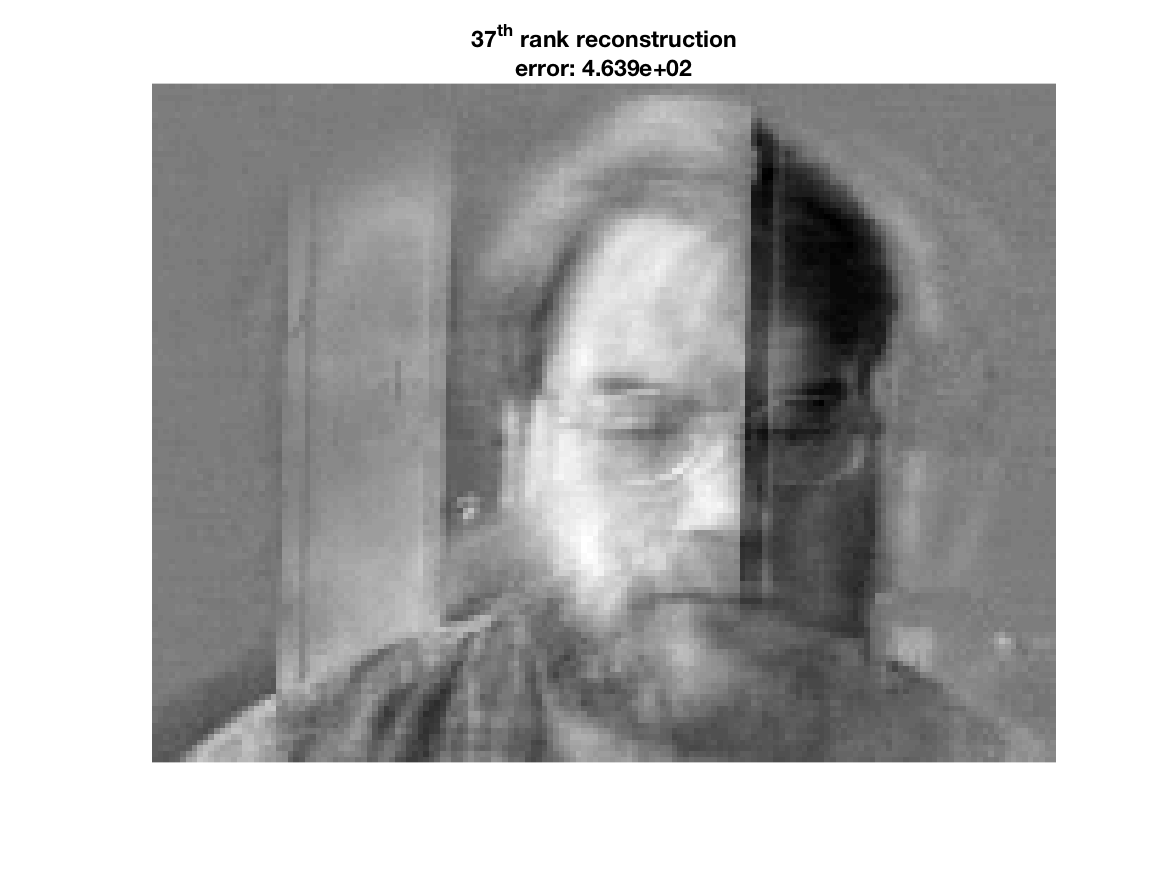
\includegraphics[trim={0cm 3.5cm 0cm 0cm},clip,width=0.6\columnwidth]{../data/rank_37_recon}
        \caption{Rank-37 Reconstruction}
        \label{fig:r37}
        \end{figure}

        \begin{figure}[H]
        \centering
        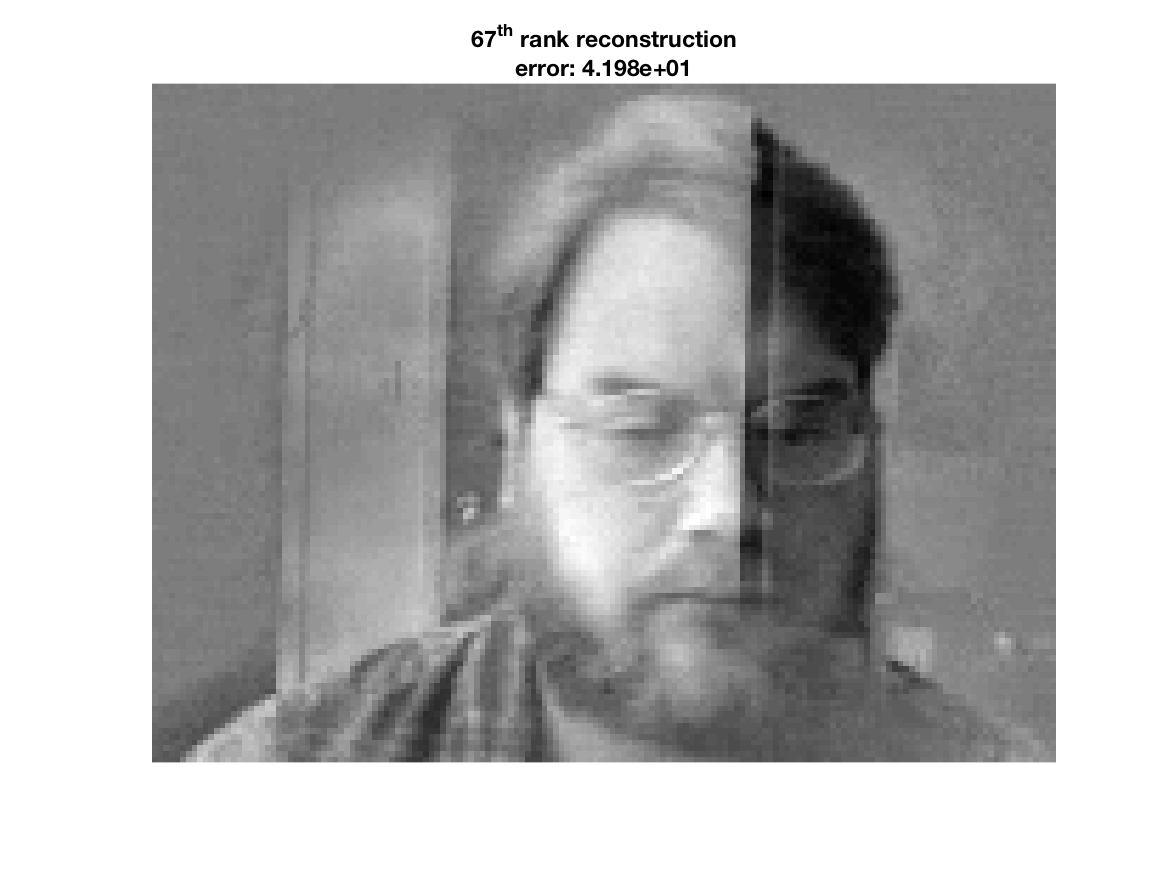
\includegraphics[trim={0cm 3.5cm 0cm 0cm},clip,width=0.6\columnwidth]{../data/rank_67_recon}
        \caption{Rank-67 Reconstruction}
        \label{fig:r67}
        \end{figure}

        \begin{figure}[H]
        \centering
        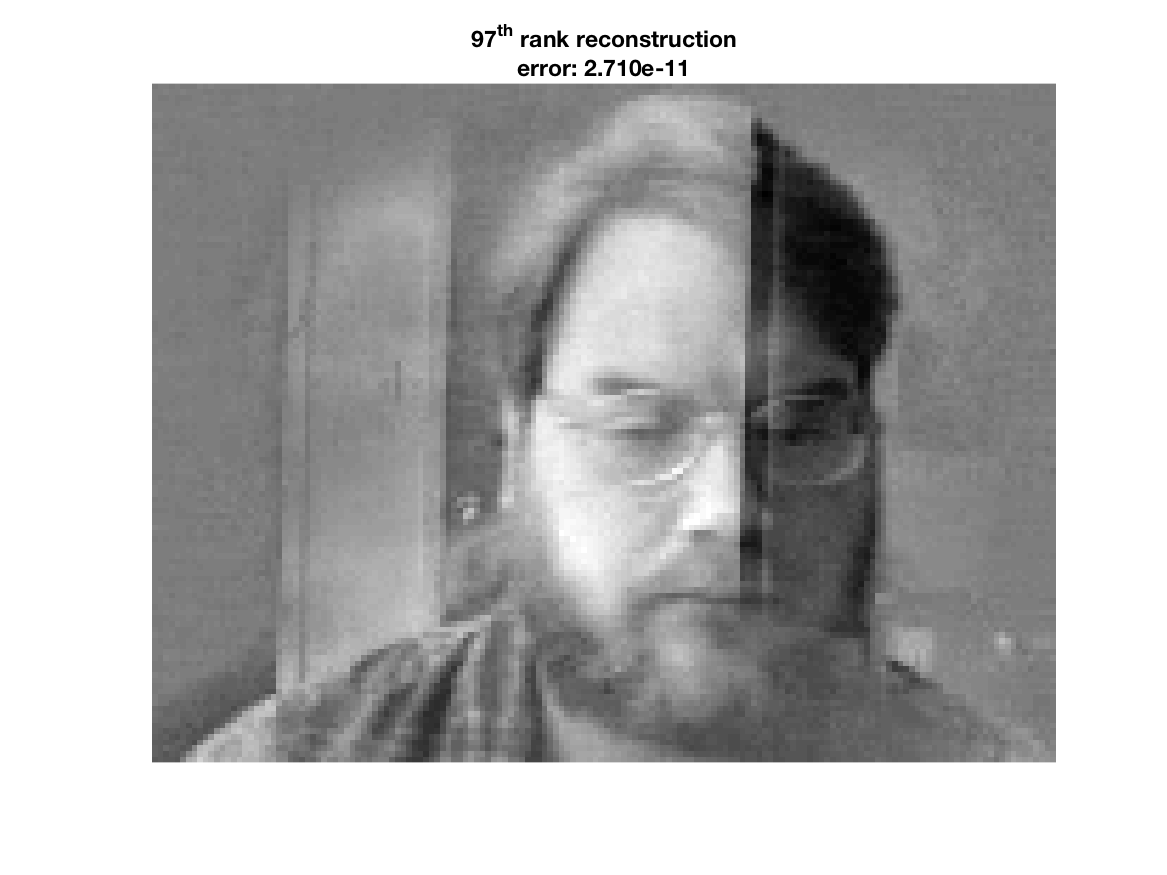
\includegraphics[trim={0cm 3.5cm 0cm 0cm},clip,width=0.6\columnwidth]{../data/rank_97_recon}
        \caption{Rank-97 Reconstruction}
        \label{fig:r97}
        \end{figure}
}

\problemAnswer{
    \begin{figure}[H]
        \centering
        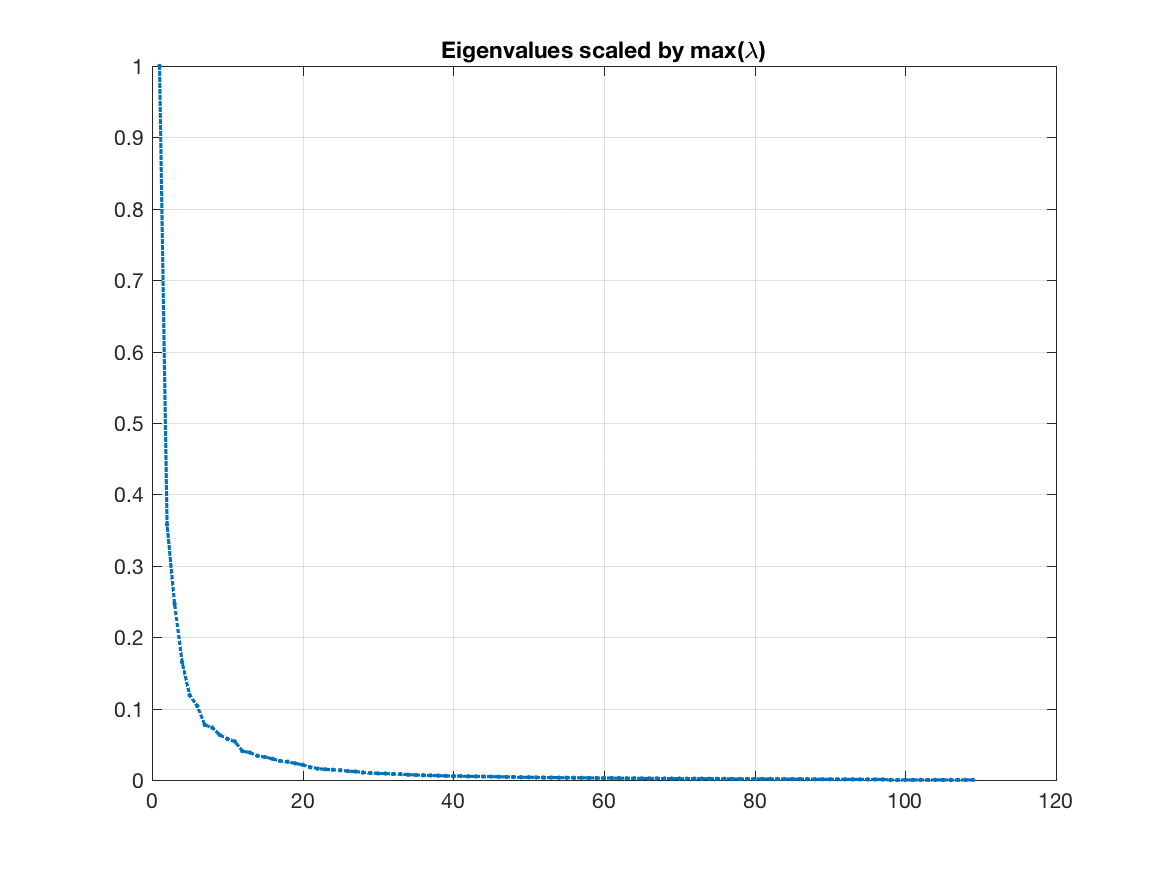
\includegraphics[trim={0cm 1cm 0cm 0cm},clip,width=0.85\columnwidth]{../data/eigvals}
        \caption{Scaled singular values}
        \label{fig:eigvals}
    \end{figure}
    

    
    \begin{figure}[H]
        \centering
        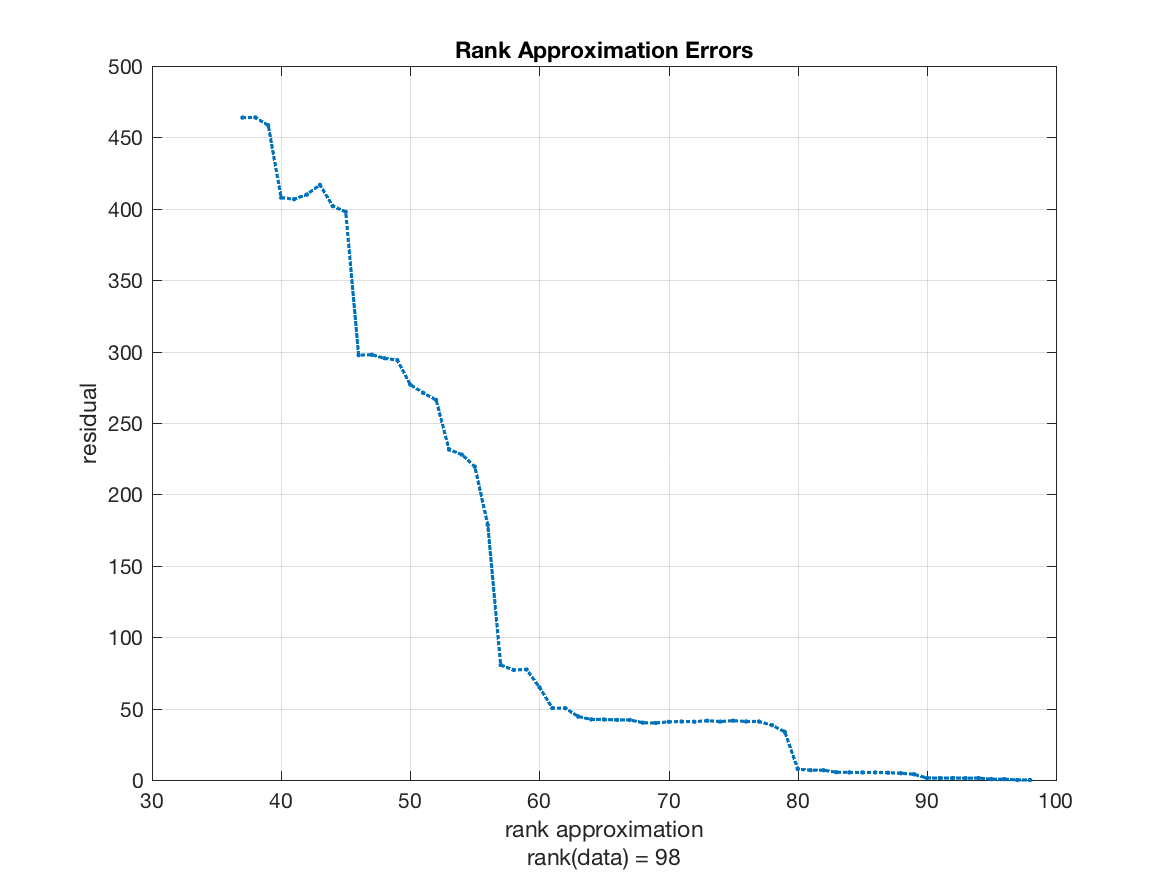
\includegraphics[trim={0cm 1cm 0cm 0cm},clip,width=0.85\columnwidth]{../data/approx_errors}
        \caption{Rank Approximation (Absolute) Errors for image 50 (rank $\geq$ 40)}
        \label{fig:approx_errors}
    \end{figure}
}
\newpage
\problemAnswer{
	Finally, we will discuss a possible classification algorithm based on this idea of best basis. We will classify a ``probe" set of data compared to a ``gallery" set, or training set. For this, we will, like usual, perform the SVD of a gallery set $X$ to get an orthonormal basis. By determining the orthonormal basis for $X$, we will then create a projection matrix $\mathbb{P}$ to project the probe set onto. 
	\\
	\\
	First, we subtract the ensemble average to make the matrices relatively on the same caxis. After projecting the probe data onto the subspace, we compare (norm of the difference) each projection with the gallery set. (Again, see the code later in this document). As shown in Figure \ref{fig:classify}, the classification works for all but one digit of our probe set (left column). The handwritten digit "8" is misclassified as a "9". We will expand on classification schemes in future projects.
    \begin{figure}[H]
        \centering
        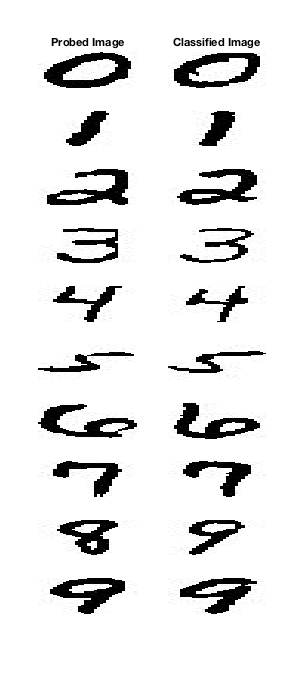
\includegraphics[trim={0cm 3cm 0cm 0.5cm},clip,width=0.45\columnwidth]{../data/classify}
        \caption{Classification results}
        \label{fig:classify}
    \end{figure}
}

\end{section}

%----------------------------------------------------------------------------------------
\newpage

\appendix

\section{Code}

\subsection{Eigenvalues and Eigenvectors}
\lstinputlisting{../Kristin_Holmbeck_HW3_Prob3.m}

\subsection{Classification}
\lstinputlisting{../classify.m}


\begin{thebibliography}{10}
    \bibitem{chang}
    Chang, Jen-Mei. \textit{Matrix Methods for Geometric Data Analysis and Recognition}. 2014.

\end{thebibliography}

\end{document}
